\newpage
\section{Gradientes de Concentração}
\label{sec:gradientes_de_concentracao}

Nesta seção o conceito de Gradientes de Concentração é explanado por meio da contextualização e definição aceca deste tema. Após isso, é apresentada uma proposta de aplicação deste conceito na área de \emph{Redes Tolerantes a Atrasos e Desconexões}.

\subsection{Contexto}

Existem particularidades nas propriedades físico-químicas quando se trabalha com compostos. Intuitivamente, exemplifica-se que, ao se fazer uma bebida - um simples suco natural - é preciso realizar a mistura de determinados ingredientes, como água, açúcar e a polpa da fruta característica pelo tipo de suco.

O processo de mistura é, na maioria das vezes, tão simples que os indivíduos nem percebem ou não levam em consideração a complexidade envolvida. Isso se deve ao fato de ser simples do ponto de vista macroscópico. Partindo de um minúsculo ponto de vista, o molecular, as moléculas de água, portadoras de propriedades particulares, são capazes de interagir com os cristais de açúcar, dissolvendo-os até um ponto de equilíbrio, que se dá quando não é mais possível continuar esse processo, ou seja, não existem mais cristais, mas sim moléculas de sacarose\footnote{Substância extraída da cana-de-açúcar e beterraba, comum em produtos alimentícios, como adoçante de alimentos e bebidas, geleias, doces e, até mesmo, xaropes.} espalhadas pela água utilizada. 

A mistura de açúcar com água possui, inicialmente, uma heterogeneidade, existindo assim um \emph{Gradiente de Concentração}, ou seja, uma diferença de concentração (os cristais de açúcar possuem maiores concentrações de moléculas de sacarose do que a água pura) entre os elementos envolvidos, dando partida ao processo de dissolução dos cristais. Esse processo ocorre até um ponto que a mistura de água e açúcar se torne uniforme, ou homogênea, de forma que não exista mais um \emph{Gradiente de Concentração}.

\subsection{Definição}

Em química, o \emph{Gradiente de Concentração} indica a alteração no valor da concentração de determinada substância por unidade de espaço. Este conceito pode ser utilizado em diversas áreas, como física, biologia e geografia. Tal gradiente é, geralmente, representado de forma gráfica \cite{concentrationGradient}.

A mistura de água com açúcar caracteriza-se por uma situação semelhante a representada na Figura \ref{agua_acucar_copo} (onde as bolinhas vermelhas representam as moléculas de sacarose e, o fluido em azul, a água).

\begin{figure}[htp!]
\centering
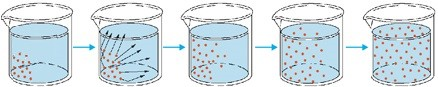
\includegraphics[width=0.80\textwidth]{figuras/cap_2/secao_2/agua_acucar_copo.jpg}
\caption{Difusão de moléculas de sacarose num copo de água \cite{concentrationGradient}.}
\label{agua_acucar_copo}
\end{figure}

É atribuído o nome \emph{difusão} ao processo representado na Figura \ref{agua_acucar_copo} \cite{concentrationGradient}. Não é objetivo deste trabalho explanar sobre as razões desse fenômeno. Em suma esse é um comportamento estocástico, natural e acontece a todo momento na natureza e no corpo humano.

Baseando-se em \cite{concentrationGradient}, é possível discretizar o processo de difusão da sacarose, obtendo o resultado visto na Figura \ref{modeculas_sacarose_agua}, onde a água pode ser vista na cor branca e as moléculas de sacarose na cor azul. É observada uma mistura gradativa do quadro esquerdo para o direita até que uma mistura quase perfeita seja alcançada.

A Figura \ref{gradiente_modeculas_sacarose_agua} apresenta os \emph{Gradientes de Concentração} para cada uma das etapas apresentadas na Figura \ref{modeculas_sacarose_agua}, baseado-se no material de \cite{concentrationGradient}. Nota-se, no gradiente à esquerda, uma grande concentração de substância na parte de baixo. A grande concentração ainda existe no gradiente do meio, mas a substância começou a se difundir para a parte superior. No último, a direita, há apenas uma cor uniforme, pois o gradiente já não existe mais, ou seja, as moléculas já se difundiram completamente.

\begin{figure}[htp!]
\centering
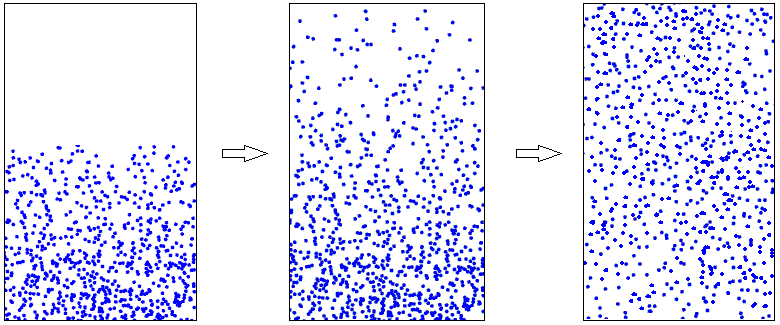
\includegraphics[width=1.0\textwidth]{figuras/cap_2/secao_2/modeculas_sacarose_agua.png}
\caption{Difusão de moléculas de sacarose num copo de água.}
\label{modeculas_sacarose_agua}
\end{figure}

\begin{figure}[htp!]
\centering
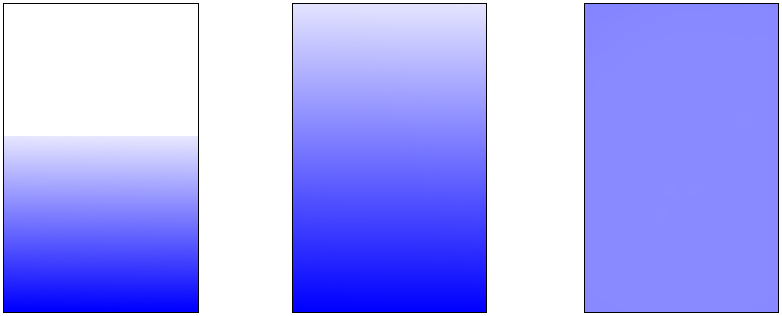
\includegraphics[width=1.0\textwidth]{figuras/cap_2/secao_2/gradiente_modeculas_sacarose_agua.png}
\caption{Gradientes de Concentração da difusão de moléculas de sacarose. A cor branca indica ausência de moléculas e, a cor azul intensa, alta concentração.}
\label{gradiente_modeculas_sacarose_agua}
\end{figure}
\newpage
\subsection{Aplicabilidade nas DTNs}

Na área de interesse deste trabalho, um \emph{Gradiente de Concentração} pode ser utilizado para representar dispositivos por unidade de área, permitindo representar regiões com muitos dispositivos como tendo maior concentração em relação a outras com menos dispositivos.

Os gradientes apresentados na Figura \ref{gradiente_modeculas_sacarose_agua} possuem uma única dimensão. Para o contexto geográfico, essa representação discretizada não traz resultados satisfatórios e, muito menos, intuitivos, principalmente pelo fato de que o mapeamento geográfico se basear em duas ou, até mesmo, três dimensões.

A Figura \ref{mapa_dispositivos} mostra um mapa com vários dispositivos distribuídos, representados por pontos verdes nomeados. Existe, no mapa, uma distribuição não uniforme de dispositivos, que é ainda mais evidenciada com a divisão em regiões de igual tamanho apresentada na Figura \ref{mapa_regioes_dispositivos}.

A concentração de dispositivos pode ser dada pela quantidade de nós de uma área dividida pela quantidade total de dispositivos da rede. A partir daí, é possível construir a Figura \ref{gradiente_mapa_regioes_dispositivos}, que representa um \emph{Gradiente de Concentração} bidimensional para o mapa inicialmente apresentado na Figura \ref{mapa_dispositivos}. A representação proporciona, de forma intuitiva, uma visualização discretizada de áreas com maior e menor incidência de dispositivos.

\begin{figure}[htp!]
\centering
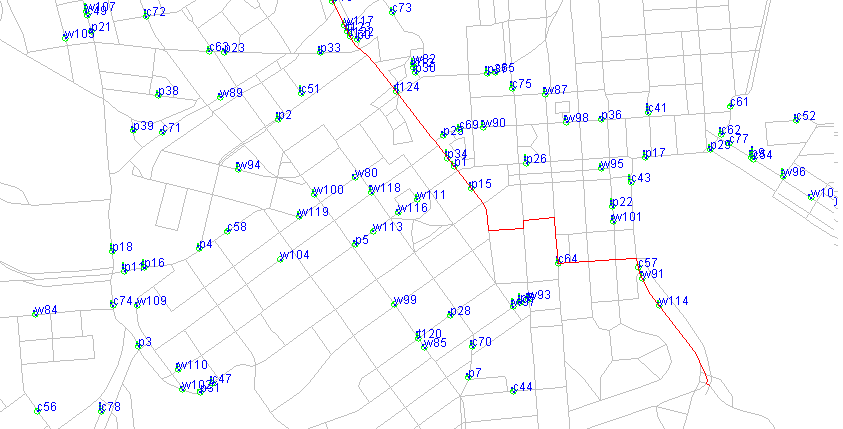
\includegraphics[width=1.0\textwidth]{figuras/cap_2/secao_2/mapa_dispositivos.png}
\caption{Mapa fictício com diversos dispositivos distribuídos por ele.}
\label{mapa_dispositivos}
\end{figure}

\begin{figure}[htp!]
\centering
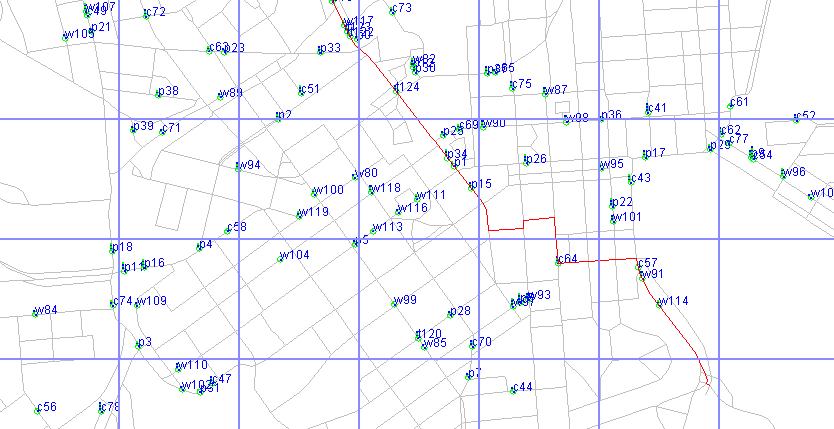
\includegraphics[width=1.0\textwidth]{figuras/cap_2/secao_2/mapa_regioes_dispositivos.png}
\caption{Mapa da Figura \ref{mapa_dispositivos} dividido em regiões de igual tamanho.}
\label{mapa_regioes_dispositivos}
\end{figure}

\begin{figure}[htp!]
\centering
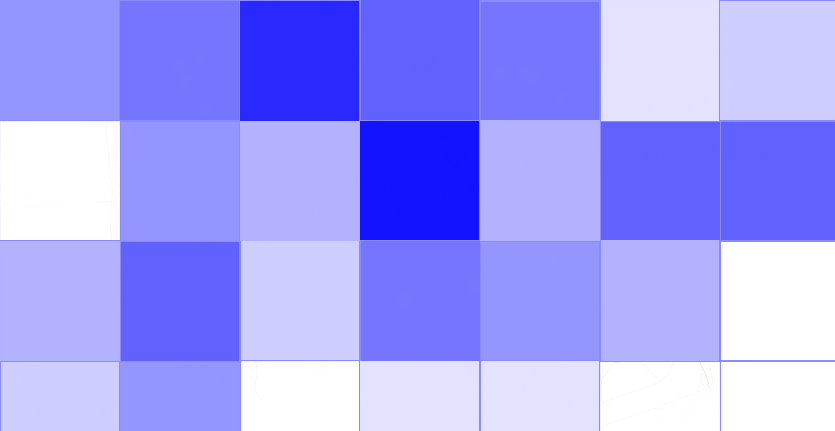
\includegraphics[width=1.0\textwidth]{figuras/cap_2/secao_2/gradiente_mapa_regioes_dispositivos.png}
\caption{Gradiente de Concentração baseado na Figura \ref{mapa_regioes_dispositivos}. A cor branca indica ausência de dispositivos e, a cor azul intensa, alta concentração.}
\label{gradiente_mapa_regioes_dispositivos}
\end{figure}

Cada região pode ser identificada e sua respectiva concentração definida por um número, inteiro ou real, responsável por indicar a intensidade desta, similar a cor. Quanto maior a concentração, maior este número e ainda maiores são as chances de encontrar algum dispositivo ao realizar uma busca. Portanto, pode-se reduzir ou aumentar a intensidade de buscas em determinadas áreas de acordo com a concentração, proporcionando um ajuste adaptativo de um importante fator no consumo de energia dos dispositivos: o intervalo de busca por dispositivos.

\subsection{Desafio}
\label{subsec:gradientes_desafios}
A representação da rede por meio de um gradiente tem como principal desafio a montagem do mesmo. O uso de técnicas de geolocalização são necessárias para o referenciamento e definição de regiões geográficas. Tais técnicas são detalhadas na Seção \ref{sec:GNSS}.

A construção do gradiente pode ser feita de forma independente entre os dispositivos que, ao entrarem em contato, trocam informações de seus gradientes numa forma semelhante a uma prosa: “Olha, eu sei que já ocorreram mais contatos na região X do que na Y, talvez isso possa ser útil para você.” e o outro responde “Legal. Como agradecimento, dar-lhe-ei as informações das regiões que já passei.”. 

Ao final de muitos contatos, os dispositivos terão um grande mapa das regiões onde eles já passaram tendo informações de localidades com maior e menor incidência de contatos, permitindo o ajuste dinâmico de fatores que influenciam no consumo de energia.